\documentclass[10pt]{article}

\usepackage{fullpage}
\usepackage{palatino}
\usepackage{amssymb}
\usepackage{graphicx,epsfig,color}
\usepackage{epstopdf}
%\usepackage{lingstyle}
\usepackage{array}
\usepackage{tabularx}
\usepackage{url}
\usepackage{lingmacros}

\setlength{\parskip}{1 mm}


\renewcommand{\baselinestretch}{1}
\newcommand{\concept}[1]{\textit{#1}}
\renewcommand{\theenumi}{\alph{enumi}}
\renewcommand{\labelenumi}{(\alph{enumi})}
\renewcommand{\theenumii}{\roman{enumii}}
\renewcommand{\labelenumii}{\roman{enumii}.}
\newcommand{\EF}{\mbox{\sf F}}
\newcommand{\WSD}{\textsc{WN$^+_{\sc F}$}}
\newcommand{\ANNO}{\textsc{EvokeDB}}
\newcommand{\MID}{\mbox{$\ |\ $}}
\newcommand{\PROB}{\mbox{\sf Pr\,}}
\newcommand{\SIM}{\mbox{\textsf{sim}}}
\newcommand{\SSIM}{\mbox{\footnotesize \textsf{sim}}}
\newcommand{\PROBS}{\mbox{{\footnotesize \textsf{Pr}}}}

\newcommand{\REF}{\textsf{BibRef}}
\newcommand{\WNP}{\textsc{WN$^+$}}
\newcommand{\WN}{\textsc{WordNet}}
\newcommand{\ARC}{arc}\newcommand{\ARCC}{Arc}
\newcommand{\NLP}{NLP}
\newcommand{\MPS}{4.85in}
\newcommand{\APP}{application}\newcommand{\APPC}{Application}
\newcommand{\ANN}{annotater}
\newcommand{\TYP}{exemplification}\newcommand{\TYPC}{Exemplification}
\newcommand{\CORE}{core}
\newcommand{\DELEGATE}{delegate}
\newcommand{\CONTEXT}{context}
\newcommand{\SIMDOM}{\mbox{$\cal D$}}


\let\origdescription\description
\renewenvironment{description}{
 \setlength{\leftmargini}{1em}
 \origdescription
 \setlength{\itemindent}{-1em}
 \setlength{\labelsep}{\textwidth}
}{\endlist}


\pagenumbering{arabic}
\renewcommand{\thepage} {D--\arabic{page}}

\newcommand{\moveup}{\vspace*{-1.8mm}}
\newcommand{\weemoveup}{\vspace*{-0.8mm}}
\newcommand{\miniskip}{\vspace*{1mm}}



\begin{document}

\begin{center}
{\LARGE{\bf Project Description}}\\*[3mm]
%{\bf SI2-SSI: Collaborative Research:\\
%The Language Application Grid: A Framework for Rapid Adaptation and Reuse}
\subsection*{IIS-RI MEDIUM: \\
Lexical Inference Patterns for Adjectives in Natural Language}
\end{center}


\section{Introduction}

Effective human communication relies on the ability of speakers to recover information that is not explicitly expressed in an utterance. 
According to \cite{graesser1985implicit}'s estimate, 90\% of what is communicated is implicit and must be inferred. \cite{grice1975logic}, in his investigation 
of the pragmatics of human communication, postulated principles of cooperative 
conversation, by which context-dependent meanings can be recognized and interpreted 
without being expressed literally or even at all. 
While some of this is due to the pragmatics of the situation and the conversation, much of such covert information can be identified as ``semantic inferences", and as such, can be associated with identifiable structural or lexical patterns in natural language.
An understanding of how speakers identify and exploit systematic covert inferences in language can enrich our models of compositionally derived inferences. 
At the same time, it can enhance the capabilities of natural language understanding systems to read beyond the surface forms of the text.

Performing such text-based inferences is one of the major goals of current {\sc nlp} research. 
This requires training machine learning ({\sc ml}) algorithms to  reconstruct the often inexplicit lexical and constructional cues in texts, just as effective human communication relies on the ability of speakers to recover information that is not explicitly expressed in utterances. 
Systems usually rely on training or development corpora that have been annotated automatically or by hand.  
These annotations are in most cases derived from lexical classes or from syntax-semantics correspondences proposed in the linguistic literature. The work proposed here focuses on lexically based distinctions. 
Previous research has mainly concentrated on the properties of verbs and nouns because the main task was information extraction, defined as identifying event or states and their participants. 
More recently, however, attention has shifted to exploiting information about the stance of the participants in the textual information exchange. 
Our work goes beyond the mere identification of entities and events and addresses the questions as to whether events have or have not occurred, might be likely to occur or not, are desirable or not, and, for entities, how their qualities compare to those of other entities. 
These questions point to a more prominent role for adjectives and adverbs. 
However, there is much less readily exploitable linguistic information available for these lexical categories, and it is less clear how their relations should be modeled. 
Moreover, the studies reported in the linguistic literature do not address the questions that motivate this proposal, because they ignore important semantic interactions between the various textual elements as well as the linguistic use of ``na\"ive'' (non-linguist) speakers. 
% non-negligible groups of speakers. 
We propose to develop a methodology that addresses these shortcomings and to validate it on three subsets of adjectives.
This approach will result in a more complete characterization of how  these adjectives are interpreted in the wild, through a better integration of lexical and corpus annotation. 
 
Our proposed research then, consists  in developing a methodology for the discovery and exploitation of systematic linguistic inferences identified with specific lexical classes in natural language. We develop this methodology in the construction of an inferential model for adjectival semantics in natural language. To this end, the specific aims of this proposal are:

\begin{itemize}

\moveup
\item Establish a model for each adjective class, combining existing background from linguistic theory with data mining techniques over large corpora to identify structure-to-inference mappings, i.e., syntactic and distributional correlates of judgments by trained annotators.
\moveup
\item Create larger labeled data sets using linguistically untrained (``na\"ive'') annotators recruited on crowdsourcing platforms, notably Amazon Mechanical Turk (AMT).
\moveup 
\item Compare judgments between trained and untrained annotators, iteratively refining experimental techniques with the goal of establishing practical methods to create larger-scale annotated corpora than is achievable using small groups of trained annotators; 
\moveup
\item Revise and enrich the model accordingly.  
\end{itemize}
\moveup
 
We concentrate on three diverse semantic types of adjectives, 
in order to both: (a) test the applicability of the methodology to different linguistic classes; and (b) to articulate just how the structure-to-inference mapping can be modeled within each lexical class. The adjective types studied are: 
(i) dimensional and evaluative adjectives with scalar values and associated scalar implicatures, e.g., \textit{pretty, beautiful, large, huge}; (ii) evidentiality adjectives, showing varying implicatures of veridicity over a clausal complement, e.g., \textit{rude, annoying, likely}, etc.; and (iii) intensional adjectives, introducing implicatures of modal subordination, e.g., \textit{alleged, supposed, so-called}. The work will result in a small Gold standard inference  corpus created by using a standard linguistic annotation effort following explicit guidelines indicating the structure-to-inference mapping for each type of adjective. But, contrary to previous studies, this standard is not the end product to be used in {\sc ml}: we will compare these baseline structure-to-inference mappings to inferential judgments made by na\"ive native speakers, such as Mechanical Turk workers (MTurkers). Our preliminary studies lead us to expect that there will be variance from the baseline. We hypothesize that an important part of this variance is caused by textual factors that are abstracted away in linguistic studies, but that are important to explain the na\"ive judgments. We will use these differential measurements in judgment (trained linguist vs. na\"ive annotator) 
to classify the implicatures according to two dimensions: how stable an inference is regardless of linguistic context; and which contextual factors contribute to blocking the expected inference. On the basis of this study, we will develop an improved gold standard and test it again with na\"ive native speakers. We will then build a model to gauge how well our distinctions explain the behavior of these speakers. Our approach will allow us to account for the interactions of different structural and lexical factors instead of seeing them as independent from each other. 

The contributions of this research are significant to the computational linguistics community in two major respects.  First, they lay the theoretical and  methodological groundwork for a large-scale annotation of adjectives in order to support automatic systems in inferencing tasks. More importantly, they contribute to a more sophisticated theory of the contribution of lexical information to inferencing. By studying the way inferences are made "in the wild" and how these differ from baseline expectations established from gold standard corpora, we can begin to identify the pragmatic factors contributing to the interpretation of lexical items in richer linguistic contexts.


 %To illustrate the utility and enabling power of this work, consider the following.
 
% 
%We propose to study the inferential properties of three classes of adjectives:  (i) dimensional adjectives, demonstrating scalar values and associated scalar implicatures, e.g., {\it pretty, beautiful, large, huge}; (ii) evidentiality adjectives, showing varying implicatures of veridicity over a clausal complement, e.g., {\it rude, annoying, likely}, etc.; and (iii) intensional adjectives, introducing implicatures of modal subordination, e.g., {\it alleged, supposed, so-called}.

Adjectives can be divided into different classes, depending on what dimensions of analysis are being used. Classic 
semantic field analysis (cf. \cite{dixon:91,lyons:77,raskin1995lexical})   categorizes the attributes denoted by adjectives according to a thematic organization, centered around a human frame-of-reference, as lexically encoded in  the language, such the following classes:\footnote{It should be noted that \cite{raskin1995lexical} , however, also discuss inferential patterns for distinct classes.}
{\sc dimension}, 
{\sc physical property}, {\sc color}, {\sc emotions}, {\sc temporal}
{\sc spatial}
{\sc value},
{\sc manner}. 

\noindent As intuitive as these classes might be for organizing aspects of the lexis of a language, they fail to provide a coherent guide to the inferential patterns associated with adjectival modification. 
An alternative approach is to 
 adopt a conceptually conservative but more formally descriptive and operational distinction, one which groups adjectives into inferential classes. \cite{amoia2006adjective} and \cite{amoia2008test}, following \cite{Kamp75twotheories} and \cite{Kamp95prototypetheory}, make just such a move, adopting a four class distinction based on inferential properties of the adjective, as illustrated below:
 
 \enumsentence{
 In the construction, [A N], A can be classed  as: \\
a. {\sc intersective}: 
the object described is both A and N. 
\\
b. {\sc subsective}: 
the object described is A relative to the set of N, but not independent of N.
\\
c. {\sc privative}: the object described is not an N, by virtue of A. 
\\
d. {\sc non-subsective}: there is epistemic uncertainty whether the object is N.  
}

\noindent These constructions   constitute  patterns that license specific inferences associated with classes of adjectives, and  can be exploited  
 in the context  of text-based inference systems, such as the RTE (\cite{amoia2006adjective}). 
This classification, however, is both too broadly defined to model the finer inferential distinctions  within each class, and too narrow to include the behavior of other adjective classes, in particular, those taking clausal complements. 
For these reasons, we have chosen to study three different classes of adjectives that  require refinements and additions to the inference patterns given above. These classes are:

\eenumsentence{
\item Scalar adjectives: both dimensional ({\it big, small}) and evaluative ({\it happy, pretty}) scalars have been categorized as subsective adjectives; 
\item Adjectives with clausal complements: adjectives such as {\it annoying} and {\it nice}, when governing clausal complements, do not fit nicely into any of the above classes;
\item Intensional adjectives: adjectives such as {\it alleged} and {\it supposed} are non-subsective, but in complex ways that are dependent on the semantics of the nominal head. 
}

%NLP has moved beyond recognizing entities and events and aims to build systems that mimic the human ability of drawing inferences from texts (we limit ourselves here to written language). This requires that they recognize not only entities and events but also the stance authors take with respect to  the described entities or events and the relations between the properties of these entities and events. 

Examples of the types of inferences we intend to capture are the following:

\begin{itemize}
 \item The {\sc pascal} Recognizing Textual Entailment (\cite{dagan+glickman+magnini:2005}) asks automatic systems to evaluate the truth or falsity of a 
statement (the Hypothesis, $H$) given a prior statement (the Text, $T$). A system must decide whether or not $H$ is true or false given $T$, as in:

\eenumsentence{
\item[$T$:] {\bf Arctic} weather swept across New Jersey. 
\item [$H$:] The Garden State experienced {\bf cool} temperatures. 
}

Apart from recognizing that New Jersey is the Garden State (information available in WordNet, see \cite{clark2007role},\cite{clark2008augmenting},\cite{clark2008using}) and the relation between weather and temperature, 
% demonstrate 
%that the semantic knowledge 
%encoded in WordNet can be harnessed to extract information that is not present 
%on the surface and measurably improve a system's performance. Thus, 
%WordNet tells us that \emph{New Jersey} 
%and \emph{the Garden State} are synonymous, increasing the probability 
%that the Hypothesis is true. (If the Hypothesis includes \emph{Empire State}, 
%systems would evaluate it as less likley to be true.) 
knowing that \emph{arctic} unilaterally entails \emph{cool} would allow a more confident evaluation of the Hypothesis. 
If Text and Hypothesis were switched, the symmetric synonymy relation between the nouns would not facilitate a correct 
evaluation of $H$, whereas the downward entailing intensity relation might lead a system to evaluate a Hypothesis containing \emph{arctic} to be false if the Text referred to \emph{cool}. An {\sc rte} system with knowledge of intensity relations among 
its adjectives is thus potentially more powerful. 

\item In order to recognize that the Text does not entail the Hypothesis in the following example, it is not enough to recognize events and their participants;  one has additionally to understand the stance the Text takes with respect to the described event:

\eenumsentence{
\item [$T$:] It is {\bf unlikely} that the attack on the consulate in Benghazi was the work of Al Quaeda.
\item [$H$:] The attack on the consulate in Benghazi was the work of Al Quaeda.
}

 
\item Concerning the third adjective class, the intensional adjectives, the effect of modifying the nominal head is the introduction of epistemic uncertainty regarding the description. 

\eenumsentence{
\item [$T$:] The police arrested the {\bf alleged} criminal.
\item [$H$:] A criminal was arrested. 
}

\noindent Hence, this inference would  be false. Now  consider the pair below:

\eenumsentence{
\item [$T$:] Archeologists discovered an {\bf alleged} paleolithic stone tool. 
\item [$H$:] A stone tool was discovered. 
}

\noindent This inference is legitimate because the epistemic scope of the adjective {\it alleged} is the adjective {\it paleolithic}, and not the nominal head itself. 
\end{itemize}

%%%
One of the resources  typically relied upon to improve automatic inferencing based on texts in natural language is supervised or unsupervised annotation of the lexical items occurring in the text. These annotations reflect directly or indirectly the inferential potential that is associated with lexical items. Some aspects of this inferential potential have been studied in detail in the linguistic literature and the computational approaches tend to take the results of these studies for granted. 
In the case of nouns, the WordNet hierarchies have proved useful; for verbs, lists of special inference patterns have been constructed starting from the work of \cite{kiparsky+kiparsky:1970} and \cite{karttunen:1971} by \cite{nairn+condoravdi+karttunen:2006}, \cite{sauri:2008phd,factbank:2009} and \cite{lotan:2012}. Information about the inferential properties of adjectives is, however, much less easy to come by. Our preliminary studies show that, for the categories of adjectives that we are interested in, the existing resources have severe shortcomings or are non-existent. One of the reasons is that the contribution of adjectives tends to be more subtle and more dependent to the rest of the linguistic context. This difficulty requires, in our view, a more careful methodology than the one that has been used up to now for syntactic and semantic lexical categorization tasks. The availability of, on the one hand, digital corpora (the biggest one being the Web itself) and, on the other, crowd-sourcing techniques to elicit the judgments of a larger and more diverse group of native speakers allow us to go beyond the narrow base that traditionally lexical studies were based on. Moreover, the development of statistical modeling techniques allow us to test theoretical hypotheses with large datasets. This should allow us to obtain better data to feed into automatic inferencing systems (such as BiuTee \cite{stern+dagan:2011} or \cite{clark2007role}). 
Although we will start from the known linguistic literature, our main effort will be focused on corpus-based analysis with the Web itself as our main corpus and on crowd-sourcing experiments. The combination of these approaches will insure that our results are representative for a larger community of users of English but they will also help us notice textual interactions that tend to be ignored in studies based on linguists' armchair intuitions.  It is important to have a solid understanding of these interactions before embarking upon a large scale annotation task: it is only if we can characterize the contribution of the targeted lexical items in its various linguistic contexts securely enough that corpus or lexicon annotation is truly useful. 
%To estimate the contribution of the factors we have isolated we will build statistical models and run them against corpus data. 

%Our methodological changes might seem minor departure from past practice but applying them jointly to the study of one adjective, \emph{lucky}, has found 1. that '{\sc np} is lucky to {\sc vp}' has an idiomatic meaning in the future that was never noticed by formal semanticists or pragmatists (discovered through the consultation of corpora), 2. that in the past lucky can be implicative and not just factive for an important subgroup of native speakers of English (discovered through the web and crowdsourcing), 3. that curated corpora only show the idiomatic meaning of lucky in the future but that the web has many examples of literal meaning in the future as well as in the past, 4. that the two meanings can often be distinguished through co-occuring structural features (discovered through crowdsourcing and model building) (cf. \cite{karttunen:2012b}). 
%and to the slides of the summer students).


\section{Theoretical Background}

\subsection{Methodological Preliminaries}

Much of current computational linguistics is based on the creation of annotated datasets focused on one or more related linguistic phenomena. Such gold standard corpora are essential for  training and tuning the statistical machine learning algorithms that are being developed to process  natural language texts. 

In the development of a gold standard corpus using rich linguistic annotation, it is typical to establish an initial model for the phenomena being studied. This  includes a triple, $M = \langle T,R,I \rangle$, consisting of a
vocabulary of terms, $T$, the relations between these terms, $R$, and their interpretation,
$I$. This is often a partial  characterization of quite extensive theoretical research in an area, encoded as specification elements for subsequent annotation. These annotations provide the features that are then used for training and testing classification or labeling algorithms over the dataset. Depending on a system's performance, various aspects of the model or related specification will be revised, retrained, and then retested. 
For this reason, we can refer to this methodology as the MATTER cycle: {\it Model}-{\it Annotate}-{\it Train}-{\it Test}-{\it Evaluate}-{\it Revise}  \cite{pustejovsky2012natural}, as illustrated in Figure (\ref{fig:matter}). 

\begin{figure}[h]
  \centering
  \scalebox{.5}{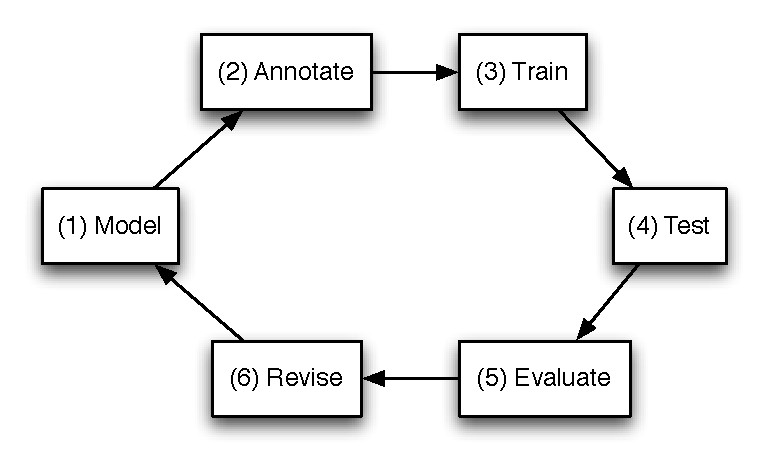
\includegraphics{matter.pdf}}
  \caption{The \textsc{matter} Methodology}
  \label{fig:matter}
\end{figure}

\noindent 
The ``Model Testing" phase of this cycle involves iterating over model development followed by subsequent testing by annotation.  	This  (Model-Annotate)$^*$ technique assumes a classic iterative software development cycle, as applied to the creation of a rich specification language to be used for linguistic annotation.  That is, as issues are encountered
with the model when instantiated in a specification and applied to data
through the annotation process, the model is revised to accommodate
these observations. 

In the present work, we propose a significant enrichment to this methodology, in order to better
model  contextual and pragmatic factors that are often ignored or down-played in this strategy. 
These involve linguistic phenomena (such as the adjective classes studied here) for which contextual factors and pragmatic effects are critical in how the annotations are interpreted.  


%% Annie's new prose
The corpora that can be annotated by trained annotators are, for practical reasons rather limited and rarely exhibit all the combinations of possibly relevant context factors. While sophisticated statistical techniques [refs by somebody who understands this better than i do] can fill in some gaps, experimental methods are necessary to supplement this shortcoming. With experiments we can achieve two goals: 
1. enrich the spectrum of interpretations that the expert annotators have given with variants of English that will not be represented by the language use of the necessarily very limited number of culturally rather similar annotators
2. allow a systematic testing of the contextually factors that the expert annotators have isolated. it is well known that isolating the factors that contribute to the perception of an inference is extremely difficult. Testing contrastive contexts with a great number of native speakers is one way to check whether the hypothesized factors are indeed the ones that are at work and whether they have been circumscribed sufficiently. For instance in FactBank, it is hypothesizing that 'NP be lucky to VP' has the meaning 'it is highly unlikely that NP VP'. We soon realized that this was too general and that this meaning is mainly found in the future. But even there more subtle factors need to isolated. In (\ref{lucky-1}), the (a) example has the highly unlikely meaning, whereas the (b) example does not (note that replacing `at least' with `in any case' makes the highly unlikely reading again more prominent).

\enumsentence{
a. Your son will be lucky to escape a jail term. \\
b.  At least your son will be lucky to escape a jail term.
\label{lucky-1}}
%% end of Annie's prose


Three key elements  play a role in the proposed work:
\enumsentence{
a. The interpretation, $I$, will focus on specific 
{\it structure-to-inference mappings} (SIMs), indicating how a given adjective type  contributes to or enables inferences associated with its embedding  syntactic contexts.  This is achieved by the conventional expert annotation. 
\\
b. The  conventional ``expert'' annotation cycle is  followed by a 
separate annotation of data constructed on the basis of the features isolated by the expert annotators but done by na\"ive native speakers.
\\
c. Iterative refinement and enrichment of the model is accomplished by comparing na\"ive and expert judgments (interpretations of SIMs for adjectives), and then revising the model appropriately. This can be referred to as {\it context-based adjudication},  revealing unseen contextual features that can then be added as model-based primitives. 
\\
d. We reach a final model when a new set of naturally occurring data receives the same annotation by the experts and the na\"ive users (modulo the dialect variation that has been detected.)
}

 
%The development of the  specification for the adjective classes follows
\noindent We proceed as follows. For each adjective class being studied (Scalar, Factive, Intensional), we establish an initial model, incorporating the appropriate SIM as the interpretation function. Expert and na\"ive annotations create corresponding gold standards, from which we perform context-based adjudication. 
 





\subsection{Scalar adjectives}
%&&Christiane edited this 12/13AM&&

Linguistic fluency entails the ability to reconstruct implicit information that is not overtly expressed in the utterance. 
%According to \cite{graesser1985implicit} estimate, 90\% of what 
%is communicated is implicit and must be inferred. \cite{grice1975logic}, in his investigation 
%of the pragmatics of human communication, postulated principles of cooperative 
%conversation, by which context-dependent meanings can be recognized and interpreted 
%without being expressed literally or even at all. 
This is true in particular 
for information accessing scales referring to gradable expressions. 
\cite{hirschberg1991theory} shows how speakers generate and interpret scalar implicatures 
in a number of specific linguistic contexts characterizing everyday, natural conversation. 
\cite{horn2000pick} establishes some intuitive scales among adjectives and notes 
that the affirmation of a weak(er) term implies the inappropriateness of a stronger term. 
For example, affirming \textit{Mary is gorgeous} implies that \textit{Mary is pretty}, an implication 
understood by the listener. 

\cite{bierwisch1989semantics} distinguishes dimensional adjectives like \textit{cold, long, high, large} 
from evaluative adjectives such as \textit{lazy, diligent, beautiful, ugly, comfortable, 
gentle, tired}. Like dimensional adjectives, these are mostly gradable but a given scale 
of evaluative adjectives tends to be more richly lexicalized, perhaps reflecting a need to specify 
qualities of everyday objects as well as a human tendency to judge people's personal, physical and intellectual traits. 
Scales for such attributes include a good number of 
adjectives that each express a different degree of intensity of the shared attribute.

For a few points on a given scale, the adjectives'
relative intensity is easy to judge intuitively. Speakers would probably agree that 
\textit{excellent} entails \textit{good}, and not vice versa.  But where exactly do 
adjectives like \textit{superb, stellar, outstanding, terrific, wonderful} fall 
on the scale? A related question is, does each adjective on a given scale 
express a different degree of a shared attribute or are some roughly synonymous for a given speaker 
or across speaker groups? 

In prior work, the direction (positive or negative) of orientation has been widely studied, 
but the degree has not. \cite{hatzivassiloglou1997predicting} extract adjectives 
with "positive" and "negative" orientation from the Wall Street Journal corpus. They show 
that conjunctions such as {\it and}
 link predominantly adjectives of the 
same orientation, whereas {\it but} links mostly adjective pairs with opposed orientation. 
Relying on the observation that the most frequent member of an 
antonymic pair has positive orientation, they assign orientation labels to the adjective 
clusters they derived. \cite{turney2003measuring} derive orientation through association 
(measured with {\sc lsa} and {\sc pmi}), based on the assumption that words with a given 
orientation co-occur with other words of the same orientation. Other related work such as 
\cite{chklovski2004verbocean} measured the relative strength of 
pairs only rather than that of all scale mates. \cite{maasmulti} learn subtle sentiment analysis 
in an unsupervised manner using a vector space model. 

%This(possibly) goes elsewhere: The answers have wide-ranging consequences 
%for the representation 
%of lexical semantics in NLP resources like WordNet. The intellectual merits of this work 
%thus are a better understanding of specific areas of the lexicon, in particular those 
%lexemes that have an evaluative component that is measurable with respect to other, 
%semantically similar lexemes. The broader impact resulting from this work are (a) shared 
%resources that enable automatic systems to better analyze and understand texts where 
%evaluation and the speaker/writer$(Bc`TE(E)I´(Bs attitudes are central components; (b) empirical data -A
%with the potential to enhance teaching materials for English as a Second Language. 

We propose an empirical large-scale and in-depth investigation of gradability among adjectives 
in different semantic domains. We cover a representative sample of twelve different semantic classes 
(\cite{bierwisch1989semantics}, \cite{frawley1992linguistic}, \cite{dixon1982have}) comprising 100 
dimensional and evaluative adjectives.  For each scale we manually identify the target lexemes using WordNet's adjective 
clusters and "similarity" relation as a point of departure. We exclude adjectives with low frequency (based on the 
BNC), as we do not expect to find enough corpus data nor reliable human judgments to 
allow us to place them on a given point on the scale. We build on, and extend, the work of \cite{sheinman2009adjscales}, who
developed a method for constructing full scales. 



%I DON'T THINK THE FOLLOWING IS RELEVANT: Antonyms
%A number of efforts focus on the extraction of antonyms from corpora, including the Web. 
%In all cases we are aware of, the goal was to extract pairs of 
%adjective antonyms or word pairs from other syntactic classes that stand in some kind of 
%semantic opposition to one another. \ref{Kamps2004} show that 
%extracted pairs can serve to disambiguate polysemous adjectives. \ref{Lobanova2010} extract 
%Dutch antonyms by first extracting lexical-semantic patterns 
%and then  searching the corpus for all occurrences of pairs linked by the patterns. 
%Unlike \cite{sheinman2009adjscales}, \ref{Lobanova2010}  do not 
%search for instances that are partially lexically filled and therefore they do not always 
%extract scale mates but merely pairwise oppositions. Results include (translated here from Dutch)
%\textit{man-woman, Bush-Putin, offer-demand} as well as many false hits, such as 
%\textit{him-orchestra}. \ref{WilliamsAnand2009} also use WordNet to build a graph that measures 
%the semantic distance between words of known polarity such as \textit{excellent-awful}. Problematically, their algorithm 
%assumes that the WordNet sense ordering reflects frequency. 
 

%% Annie's stuff


\subsection{Inferences of predicative adjectives with clausal complements}

Another class of adjectives that are a rich source of inferences are predicative adjectives with clausal arguments (\emph{that} {\sc s}, \emph{to} {\sc vp}, or \emph{ing} complements). The class comprises hundreds of adjectives whose use communicates an agent's epistemic stance on the likelihood of the (non-)occurrence of the eventualities described by their clausal argument. Some of the adjectives convey, in addition, an emotive or evaluative attitude of the agent. As we discuss below, the inferential classification of this class poses interesting challenges.
%% With these adjectives the inferences are about the (likelihood of the) occurrence or non-occurrence of the events or states described in the embedded clauses.
%It is fair to say that WordNet doesn$(Bc`QU(B pay much attention to the predicative use of adjectives. Most examples show the attributive form.  When one is interested in inferences, however, the predicative use can be revealing because 
 %% There are hundreds of such adjectives but, as we will discuss, their inferential classification is not always easy.
%%The class comprises hundreds of adjectives but, as we  discuss below, their inferential classification is not always easy.

%%These inferences will not depend on the adjective alone but need to take at the very least the syntactic frame into account. 
The relevant agent as well as the type of inferences that arise depend
on both the adjective and its syntactic frame.  The agent with the
implied epistemic stance is sometimes the speaker/writer and sometimes
the referent of the subject of the predicative construction (the
`protagonist').  For instance, \textit{John is sure that Bill left}
ascribes the belief that Bill left to John (the protagonist) and
leaves open what the writer thinks, whereas \textit{John is sure to have
left} ascribes a belief to the writer. Similarly, the syntactic frame
alone does not suffice to determine the type of inference. For
instance, not all adjectives that fit into the [It is {\sc adj} that
  {\sc s}] pattern behave the same way, as shown below.  Thus, if one
is interested in inferences that can be drawn on the basis of
linguistic form, one has to consider lexical items together with their
syntactic patterns.

There is no generally accepted classification of predicative adjectives taking clausal complements on either syntactic or semantic grounds, but three broad classes have been distinguished based on their epistemic inference patterns. 

\vspace{-1.0em}
\paragraph{1. Factive adjectives} These are adjectives  implying that the author is committed to the factuality of the state of affairs described in the complement even when the matrix clause is negated or questioned. They are traditionally analyzed as presupposing the truth of their complement.
Take, for example, (\ref{annoying1}).
%the following sentence. 
 \vspace{-0.5em}
\enumsentence{
It is annoying that people post stuff that no one cares about on the web.
\label{annoying1}}
\vspace{-0.5em}
 
 
\noindent From (\ref{annoying1}), the reader infers that the author 
presents 
%believes 
as true the proposition 
that people post stuff that nobody cares about on blogs.
This inference is derived directly from the semantics of the adjective {\it annoying}, when used in such a construction. 
Neither negation nor questioning  changes the veridicity of the \emph{that }clause, as illustrated in (\ref{factive}).  The focus of the question in (\ref{factive}b) is the evaluation of the \textit{that}-complement as annoying or not.
 \vspace{-0.5em}
\enumsentence{
a.  It isn't annoying that people post stuff that no one cares about on blogs. 
\\
b. Is it annoying that people post stuff that no one cares about on blogs?
 \label{factive}
}
 \vspace{-0.5em}

%% \noindent
%% Both these sentences still carry the inference that \emph{people post stuff that no one cares about on blogs.}
%% Not all 
%% adjectives that fit into the  [It is {\sc adj} that {\sc s}] syntactic pattern behave the same way, as shown below in our discussion of the second class, nor is this  the only pattern that predicative adjectives with complements allow. 

The only comprehensive study of factive adjectives was done by Norrick in \cite{norrick:1978}. Norrick proposed two big subclasses : emotive (e.g. \textit{sad}) and evaluative (e.g. \textit{stupid}) adjectives. The empirical picture , however, is more complicated and the status of the factuality inference varies among speakers, as reported in \cite{csli-gang-cssp13} and discussed below.
%%As we will illustrate below he does not take all the relevant variables that influence the inference in consideration. 

%% With \emph{annoying}, for example,  neither negation nor questioning  changes the veridicity of the \emph{that }clause, as illustrated in (\ref{factive}). 
%%  \vspace{-0.5em}
%% \enumsentence{
%% a.  It isn't annoying that people post stuff that no one cares about on blogs. 
%% \\
%% b. Is it annoying that people post stuff that no one cares about on blogs?
%%  \label{factive}
%% }
%%  \vspace{-0.5em}

%% \noindent
%% Both these sentences still carry the inference that \emph{people post stuff that no one cares about on blogs.} This is not the case, however,  with \emph{certain}:
%%  \vspace{-0.5em}
%% \enumsentence{
%% a. It is certain that people post stuff that no one cares about on blogs.
%% \\
%% b. 
%%  Is it certain that people post stuff that no one cares about on blogs?  
%% \label{certain}
%% }
%%  \vspace{-0.5em}
%% In (\ref{certain}b) it is the \textit{that}-complement that is questioned, whereas with \emph{annoying} it is the evaluation of the \textit{that}-complement as annoying that is the focus of the question. 
%% It would be of use to know which adjectives behave like \emph{annoying} and which ones behave like \emph{certain}. 

%% Different subcategorization frames can also carry different implications. Consider the following two sentences. 

%% % \vspace{-0.5em}
 
%% \enumsentence{
%% John is sure that Bill left.
%% \label{sure1}}
%% \vspace{-1.0em}

%% \vspace{-1.0em}
%% \enumsentence{
%% John is sure to have left. 
%% \label{sure2}
%% }

%\vspace{-1.0em}

%% \noindent
%% Whereas (\ref{sure1}) ascribes the belief that ``Bill left" to John (the protagonist) and leaves open what the writer thinks, (\ref{sure2}) ascribes an opinion to the writer.


%% If one is interested in inferences that can be drawn on the basis of linguistic form, one has to consider lexical items together with their syntactic patterns.


%Before going into the details of the inferential information that the language provides us with here, it is useful to make a distinction between \emph{factuality}, (where a state of affairs obtains or has obtained in reality) and the author's commitment to this factuality, which can be total or probabilistic, which we will call \emph{veridicity} in what follows. When reading (or hearing) a statement, the reader has to decode the author's commitment. We call this the {\sc riv} (\emph{reader inferred veridicity}) and to evaluate the probability of the factuality of a state of affairs given all of his/her information. We will call this final evaluation, the \emph{reader inferred factuality ({\sc rif})}. As we are considering textual information we have no direct knowledge of the factuality of a state of affairs as such. The choice of textual devices, however, gives us important indications about what the author considers to be the case or not. 
%%The reader/hearer exploits these devices together with world knowledge of all types to calculate his/her own {\sc rif}, which typically with be a probability estimation: texts/oral communications are used to acquaint people with factuality's that they have not directed witnessed and about which they might never acquire absolute certainty. 
%In this proposal we are mainly concerned with {\sc rivs} because that is the aspect that seems reasonable invariant over different readings of a same text by different people in different circumstances. The {\sc rifs} will vary given they will take into account the reader's evaluation of the author's reliability, the reader's prejudices and prior knowledge. They are not based on textual inferences alone.
%We make the not too controversial assumption that modeling how people understand texts will be an important to build systems that do automatic inferencing. But we are not assuming that such systems are modeled as a person. A person will often disambiguate an expression without even being aware of there being an ability. In a system it might often be better to keep a weighted ambiguity, leaving a final factuality judgment either until more information becomes available or until an other external decision criterion comes into play.
%Veridicity information on its own is important e.g. for high quality translate but we also want to know what the probability is that a message is understood as conveying that a particular event has happened or not. We assume that there is a correlation between the speaker's intention and the reader's interpretation but we do not expect them to be identical and we need to measure how much understanding the author's intentions contributes to the ultimate reader judgments.  One study that addresses this problem in part is De Marneffe et al.  Their study focusses on the contribution of verbs. It shows that there are strong correlations in most cases but not in all. The most important exceptions they see are the effects of verbs of saying where there is a clear difference between the commitment of the protagonist and that of the author. These cases are rare with adjectives. Their second important class are modal verbs. It might be the case that degree of certainty adjectives behave similarly to those. 
%% There is no generally accepted classification of predicative adjectives taking clausal complements on either syntactic or semantic grounds but we can distinguish two broad types of inference patterns: 
%\vspace{-1.0em}
%%\eenumsentence{
%% \item \emph{factive} adjectives as illustrated above in (\ref{factive}). They imply that the author is committed to the factuality of the state of affairs described in their complement even if the matrix clause is negated or questioned.
%%  \vspace{-0.5em}
%% \item \emph{certainty} adjectives that directly assert the degree of certainty that the speaker, or a protagonist, ascribe to the complement, as illustrated in (\ref{certain}). When these adjectives express absolute certainty of absolute denial of the truth of the embedded clause, they give rise to logical entailments; they are \emph{implicative}. Implicatives come in different varieties, as illustrated in table 1. When they do not express absolute certainty, they are part of the means an author uses to indicate the probability that (s)he attaches to the factuality of the state of affairs expressed in the embedded clause. In this study, we follow \cite{sauri:2008phd} and approximate this probability by the following scale: {\sc ct}+ (certain), {\sc pr}+ (probable), {\sc ps}+(possible), {\sc u} (none), {\sc pr}- (improbable), {sc pr}- (impossible) and {\sc ct}- (certainly not).
%% }

%% A supplementary factor that plays a role in certain cases, as illustrated above (\ref{sure1} and \ref{sure2}), is whether the judgment is that of the writer or is attributed by the writer to a protagonist in the sentence or discourse, e.g., the subject of the sentence with a predicate of saying. 

\vspace{-1.0em}
\paragraph{2. Certainty  adjectives} These adjectives directly assert the degree of certainty that the write, or a protagonist, ascribes to the complement, as illustrated in (\ref{certain}).

\vspace{-0.5em}
\enumsentence{
a. It is certain that people post stuff that no one cares about on blogs.
\\
b.  It is not certain that people post stuff that no one cares about on blogs.\\
 c. Is it certain that people post stuff that no one cares about on blogs? 

\label{certain}
}
 \vspace{-0.5em} In (\ref{certain}c) it is the
 \textit{that}-complement itself that is questioned, and
 (\ref{certain}b) has the opposite inference from that of
 (\ref{certain}a).  Structure-inference patterns for these adjectives
 then would need to distinguish between positive contexts, negative
 contexts and questions.


%Like \textit{certain}, 
Some of the adjectives in this class express absolute certainty or absolute denial of the truth of the embedded clause, and hence give rise to logical entailments; they are \textit{implicative} (\cite{karttunen:1971}). Others, such as \textit{possible, probable, impossible, improbable}, do not express absolute certainty but constitute a means for the author  to indicate the probability that (s)he attaches to the factuality of the state of affairs expressed in the embedded clause. In this study, we follow \cite{sauri:2008phd} and approximate this probability by the following scale: {\sc ct}+ (certain), {\sc pr}+ (probable), {\sc ps}+(possible), {\sc u} (none), {\sc pr}- (improbable), {sc pr}- (impossible) and {\sc ct}- (certainly not).

Apart from the adjectives that express an epistemic stance directly, there are adjectives expressing other modalities that have epistemic consequences. These include \textit{able (to), unable (to), willing (to), not willing (to)}, also \textit{unthinkable (that), unbelievable (that)}. Their negative versions may carry negative entailments (\textit{unable to VP} implies that the situation 
described  by the VP complement did not come about), while their positive versions lead to the expectation that the situation described by the complement has occurred or will occur but without warranting an entailment relation.

\vspace{-1.0em}
\paragraph{3. Adjectives with no epistemic implications}
These adjectives fall into several subclasses, e.g. \textit{easy} adjectives, dispositional adjectives such as \textit{afraid (to), keen (to)}, mandative adjectives such as \textit{important (to), essential (to)}, etc. While these do not lead to logical entailments, some of them invite the \textit{inference} that the writer thinks that their complement is factual or at least very likely to have happened. The factors that trigger these invited inferences need further study.





%% \medskip
%% \vspace{-1.0em}
%% \begin{table}
%% \caption{implicative and factive patterns}
%% \centering
%% \begin{tabular} {l l l}
%% \hline
%% Implicative & example & illustration\\ \hline
%% two way & manage to & {\scriptsize If Kim manage to do it, Kim did it; If Kim didn't manage to do it, Kim didn't do it.}\\ 
%% & forget to & {\scriptsize If Kim forgot to do it, Kim didn't do it; If Kim didn't forget to do it, Kim did it.}\\
%% one way & force to & {\scriptsize If Kim forced Sandy to do it Sandy did it.}\\
%% & refuse to & {\scriptsize If Kim refused to do it, Kim didn't do it. }\\
%% & attempt to & {\scriptsize If Kim didn't attempt to do it, Kim didn't do it.}\\
%% & hesitate to & {\scriptsize If Kim didn't hesitate to do it, Kim did it.}\\
%% \hline
%% Presuppositional & example & notation\\ \hline
%% factives  &forget that	&  {\scriptsize If Kim forgot that the stove was on, the stove was on.}\\
%% counterfactives & pretend that	& {\scriptsize If Kim pretended that the stove was on, the stove was not on.}\\
%% \hline
%% Neutral & want to & no implication \\
%% \hline
%% \end{tabular}
%% \label{implicatives and factives}
%% \end{table}
 
 
%% The most common type of inferential pattern for this class is the factive one (illustrated above in \ref{factive}). It is also the most studied. \cite{norrick:1978} is to our knowledge the most extensive study of adjectives taking \emph{that} and \emph{to} clauses. \cite{wilkinson:1970} and \cite{barker:2002} are less extensive studies with claims about factivity.
In addition to the extensive study of factive adjectives in \cite{norrick:1978},
there are the more limited studies in \cite{wilkinson:1970} and \cite{barker:2002}. Implicative patterns (\cite{karttunen:1971}) and degree-of-certainty adjectives are only mentioned in passing in the literature. \cite{mindt:2011} looks at the syntax of 51 frequent adjectives taking \emph{that }clauses in the BNC but without any attention to the semantics.\cite{vanlinden+davidse:2009} report on a corpus study of deontic-evaluative adjectives concentrating on \emph{important, essential, crucial} and \emph{appropriate, proper and fitting}. They attempt to distinguish between propositional and mandative uses (the former describes a state of affairs, whereas the latter intends to bring a state of affairs in existence or to prevent it from coming into existence) and show that the correlation between the mandative use and the subjunctive is not absolute. The syntax of  \emph{eager} and \emph{easy} adjectives has been well-studied. But not much attention has been given to their semantics. We ignore the literature on these classes as it is irrelevant to our purposes. We are not aware of any computational work that focuses on any of these adjective classes. 

Pilot studies we have conducted on various subclasses of adjectives with clausal complements have revealed  that their inferential behavior is dependent on fine-grained structural and contextual factors. 
% conditioning factors . 
%We classify the patterns on the basis of their surface syntax, abstracting away from linguistic arguments about argument status.
 An exhaustive list of all patterns cannot be given in the confines of this proposal. We discuss some of our observations to illustrate that getting a proper inferential classification  needs further, systematic study.



\vspace{-1.0em}
\paragraph{a. Impersonal constructions of the type [it be ADJ (of NP) to VP]}
 Adjectives in this syntactic pattern can belong to any of three inferential classes described above. 
\cite{norrick:1978} lists several hundred as factive. But even among those 
the situation is more complicated. A sentence like \textit{It was audacious of John to make a trip around the world} readily gets a factive interpretation but one like \textit{It is audacious of anyone to make a trip around the world} very rarely.
Our preliminary investigation of the evaluative adjectives among these shows that a factive interpretation reliably arises only in the past tense with a specific \textit{of NP}. For this case we can have the structure-to-inference mapping in (\ref{sti-factive-eval}).

\vspace{-0.5em}
\enumsentence{\label{sti-factive-eval}
$ [ \mbox{ it was } \mbox{ \textit{ADJ}}_{\mbox{\textit{eval}}} \mbox{ of } \mbox{ \textit{NP}}_{\mbox{\textit{spec}}} \mbox{ to } \mbox{ \textit{VP} } ] \; \vDash \; \mbox{ \textit{NP}}_{\mbox{\textit{spec}}} \mbox{ \textit{past} } \mbox{ \textit{VP}} $
}
\vspace{-0.5em}

\noindent
The other variants of the pattern (present tense, non-specific \textit{NP} or no \textit{of NP}) allow for much variation in interpretation.

Adjectives without epistemic entailments may nevertheless give rise to interpretations where a high degree of probability is ascribed to the truth of the complement. For instance, \textit{It was essential for researchers to collect accurate information} is judged by Mechanical Turk workers to be factual for more than 50\% of them and probable for another 35\%. 
%(other choices were unknown, 50-50, certainly not and probably not). 

Our preliminary results thus suggest that for this syntactic pattern there are several subclasses of the three broad, traditionally recognized classes, for which the exact conditioning factors have yet to be identified.

\vspace{-1.0em}
\paragraph{b. Personal constructions of the type [NP be ADJ to VP]}
We have discovered that factive adjectives in this frame are implicative under certain circunstances for many people (\cite{csli-gang-cssp13}). 
The preferred interpretation of \textit{I wasn't stupid to send money} is that no money was sent. We looked at 60 occurrences of \textit{is/was stupid to} in the enTenTen English corpus, one of the only curated corpora that includes blogs, and found that 25 were clearly factive, 23 clearly implicative and 12 either unclear or part of a different construction. This result was corroborated by a pilot experimental study, which showed that for a sentence such as \textit{Kim was not stupid to waste money} 66.7\% of the subjects give an implicative interpretation (when given the choice between implicative, factive and don't know). Similar results obtain with \textit{clever}.
This pattern is clearly dependent on extra-linguistic factors: for \textit{Kim was not stupid to save money}, we get 78.6\% in favor of a factive interpretation. Previous theoretical assumptions, however, would have predicted only the factive interpretations in both cases.

%%Our preliminaries studies suggest that there is wide variation among these adjectives wrt the acceptability of the implicative reading. 

\vspace{-1.0em}
\paragraph{c. Personal and impersonal constructions with a \textit{that}-complements} 
Our preliminary investigation suggests that \textit{that}-complements of factive adjectives give rise to rather solid factive interpretations but a more detailed study needs to be done.  A preliminary classification of these adjectives is available on-line (\cite{faust-adj-pol-lex}). A structure-to-inference mapping corresponding to an impersonal syntactic frame is given in (\ref{sti-factive}).
\vspace{-0.5em}
\enumsentence{\label{sti-factive}
$ [\mbox{ it be } \mbox{ \textit{ADJ}} \mbox{ that } S \; ] \; \vDash \; S$
}
\vspace{-0.5em}

%The distinction between writer and protagonist based inferences is made most clearly in Sauri (2008) but that study contains little information about adjectives and some of the categorizations seem to be wrong. 
%He treats many more adjectives as factive than seems warranted. 

%% The nature of the available data calls for several comments for the motivation of our research plan. 
%% \vspace{-1.0em}

%% \begin{enumerate}
%%   \item The linguistic classification encodes veridicity or, if interpreted from the reader's point of view, reader inferred veridicity, but the judgments are made by a narrow set of linguists. There are no data reflecting the judgments of na\"ive native readers. Specifically with respect to degree-of-certainty classes, linguists assume that the 'literal' meaning of the adjective reflects the degree of certainty. This needs to be tested.
%% \vspace{-1.0em}

 
%%   \item Linguists choose their examples so as to control for variations in e.g. tense or the presence of absence of the syntactically optional arguments, that might obscure the judgements they are interested in. The studies above are based on classic linguistic tests where the test sentences are typically in the past and the relevant arguments have all specific referents. But our preliminary experiments show that there is a big difference in the way people interpret a sentence such as
%% \emph{It was annoying of Bill to leave early}
%% and a sentence like
%% \emph{It is annoying to leave early}. There is no explicit study of the factors that might override the factivity interpretation of a so-called factive adjective. It is important to understand these factors (genericity  in the case illustrated\footnote{For treatment that dovetails with our preliminary findings, see \cite{mathew+katz:2009}}) if one wants to predict the way a sentence will be interpreted in a running context. We will first check the linguistic judgments with their restrictions by submitting them to na\"ive native speakers and then broaden the investigation by submitting variants that do not respect these constraints. 
%% \vspace{-1.0em}

%%   \item Language variation. For some of the adjectives that are classified as factive, one finds on the web examples that clearly imply a non-factive interpretation. For instance, we find instance such as 
%% \emph{This is my first trip to Italy, so I was not brave to venture out alone},
%% where the implication is clearly \emph{I did not go out alone}. The adjective is not used as a factive but rather as a two-way implicative. A preliminary study indicates that these readings are accepted as unexceptional by a sizable minority (20\%) of native American speakers.   
%% In some cases we can even distinguish two rather different meanings for a same construction. This is the case for \emph{lucky} in the future tense, as discussed in \cite{karttunen:2012b}. 

 
%% We will ask na\"ive native speakers about their judgments, both testing for their passive acceptance of the various patterns and for their willingness to produce such patterns. 

 
%% \end{enumerate}

\subsection{Intensional Adjectives}





  The third adjective class we examine for their inferential properties is  the
set of 
non-subsective intensional adjectives. 
%Recall that intersective adjectives such as {\it carniverous} have the following behavior:
% 
% \enumsentence{
% $
% \| A \; N \; \| \; = \; \| A \| \cap \| N \| $
% }
% \noindent
% Subsective adjectives, on the other hand, such as {\it big}, can be modeled as follows:
% 
% \enumsentence{
% $\; \| A \; N \| \subseteq \| N \| $
%  }
%
The intensional adjectives can be split into privatives and non-subsective. 
Privatives, such as {\it fake} or {\it pretend}, can be analyzed as follows:
\vspace{-0.5em}
 \enumsentence{
 $
 \| A \; N \| \cap \| N \| \; = \; \emptyset $
 }
\vspace{-0.5em}

\noindent
Intensional non-subsective adjectives introduce an epistemic uncertainty for the elements within their scope. 
Examples of  this class include \emph{alleged},
\emph{supposed}, and \emph{presumed}, and they call 
into question some predicative property of the nouns they modify. Following \cite{Kamp95prototypetheory}, no informative inference is associated with this construction:
\vspace{-1.0em}
\enumsentence{
a. $  [ A \; N]  $ (alleged criminal)
\\
b.  $\nvDash  \;  N  $
}
\vspace{-0.5em}

\noindent However, contrary to what is claimed in \cite{amoia2006adjective}, non-subsective adjectives do appear to license specific inferences when examined in a broader context than the [A N] construction usually studied. From preliminary corpus studies of this class\footnote{The initial corpus has been collected from directed CQL queries over  two Sketch Engine corpora, Ententen12 and BNC. Three sentence ``snippets" have been compiled from this source.}, several distinct patterns of inference emerge. While the typical resulting composition entails  uncertainty of 
 whether the nominal head belongs to the mentioned sortal, (\ref{ex:alleged_criminal}) below, there are many contexts where the epistemic scope is reduced to  a modification or additional attribution of the nominal head, as shown in  (\ref{ex:alleged_paleolithic_tool}). 

\vspace{-0.5em}
\eenumsentence{
	\item The \textbf{alleged criminal} fled the country.
	\label{ex:alleged_criminal}
\vspace{-0.5em}
	\item Archeologists discovered an \textbf{alleged paleolithic tool}.
	\label{ex:alleged_paleolithic_tool}
}
\vspace{-0.5em}

\noindent 
In Example (\ref{ex:alleged_criminal}), the adjective \emph{alleged} calls into question the predicative property of `criminality' of the \emph{criminal}. When a predicative property is called into question by adjectives of this class, are
there any systematic inferences to be made about the semantic field? E.g., is the semantic field still guaranteed to be some hypernym of
\emph{criminal}? Even if the individual does not belong to the set of
``criminals'', it does still seem to belong to the set of ``persons''. In
example (\ref{ex:alleged_paleolithic_tool}), contrastively, at least under one
interpretation, it is whether the \emph{tool} is \emph{paleolithic} or not that
is called into question: i.e., the object belongs to the set of ``tools''
regardless if it is truly \emph{paleolithic} or not.
This inference is schematically represented below.

\vspace{-0.5em}
\enumsentence{
Given the construction $[A_{int} \; N]$, where $A_{int}$ is {\it alleged, ...}, then: \\
a. $[ A_{int}\; N ] \; \nvDash \; N$ \\
b. $[ A_{int} \; A_2\; N ] \; \nvDash \; A_2$\\
c.   $[ A_{int} \; A_2\; N ] \vDash \; N$
\label{AAN}
}
\vspace{-0.5em}


\noindent 
Such an inference pattern is subject to contextual variables, many of which are not available to sentential compositional mechanisms, but some constraints can be identified. For example, the closer the head noun is to a sortal base level category, such as  {\it bird}, {\it table}, or {\it tool}, the more likely the inference in (\ref{AAN}) will go through. 
Consider the examples below:

\vspace{-0.5em}

\enumsentence{
a. The store bought an alleged antique vase. \\
b. 
The researcher found an alleged Mozart sonata. 
\label{AAN2}}

\vspace{-0.5em}


\noindent These cases make it clear that the epistemic uncertainty in (\ref{AAN2}) involves an additional aspect of the NP,  beyond the unassailable characteristics of the entailed head. That is, the object is clearly a vase (in (\ref{AAN2}a)) and demonstrably a sonata (in (\ref{AAN}b)). Such evidence, however, will not always be available within the composition of a sentence, but will be derivable from context (if at all).  We will refer to the canonical inference in (\ref{AAN}a) as the ``Wide-scope reading'', and the inferences in 
(\ref{AAN}b-c) as the ``Narrow-scope reading". 

Another interesting distinction emerging in the basic [A N] construction with intensional adjectives is  one based on the   type of the nominal  head. 
The most common semantic types occuring in the corpus are shown below, along with apparent scoping behavior. 

\vspace{-0.5em}
\enumsentence{
a. {\sc event nominal}: 
{\it violation}, {\it misconduct}, {\it murder}, {\it assault}. The more specific nominal descriptions carry greater inferential  force for the hypernym. That is, {\it murder} suggests inference of a death. 
\\
b. {\sc agentive noun}: {\it collaborator}, {\it
perpetrator}, {\it murderer}, {\it criminal}. Epistemic scope is over the
entire sortal.  The canonical form, ``the alleged criminal". 
\\
c. {\sc undergoer noun}: {\it victim}.  While not
always the case, the scope is narrowed to a modification of the event: For example,  ``the alleged victims of  Whitey Bulger". 


\label{headtypes}}
\vspace{-0.5em}



Consider the sentences in (\ref{types1}), where {\it alleged} is modifying an event nominal. 

\vspace{-0.5em}
\enumsentence{
a. He denies the alleged assault on the police. 
\\
b. The greatest number of	 alleged	 violations occurred in California. \\
c. He's been charged in connection with the  alleged murder of John Smith, whose mutilated body ...

\label{types1}}
\vspace{-0.5em}

\noindent The inferences associated with (\ref{types1}a-b) follow from the template in (\ref{AAN}a). For 
sentence (\ref{types1}c), however, we need to infer that there was, in fact, a killing, although it is uncertain whether it was a murder. This requires the inference rule below, where the hypernym of the event nominal is infererable from the context.

\vspace{-0.5em}
 \enumsentence{
Given the construction $[A_{int} \; N]$, where $N$ is an event nominal, with certain feature, then: \\
a. $[ A_{int}\; N ] \; \nvDash \; N$ \\
 $\vDash$ $N'$  where $N \subseteq N'$
}
\vspace{-0.5em}

\noindent We refer to this inference rule as the ``Hypernym reading". 
Similar remarks hold for undergoer nominals in some contexts, where the scope of the intensional adjective can be lowered to a modification of the event description. This is illustrated  below, in (\ref{victim}b).  

\vspace{-0.5em}
\enumsentence{
a. Testimony will be heard from the alleged victim in court. 
 \\
 b. The families of two alleged victims of James "Whitey" Bulger have received compensation. 
\label{victim}}
\vspace{-0.5em}


\noindent Sentence  (\ref{victim}a) behaves according to the canonical template, while  (\ref{victim}b) involves a narrower scope of the epistemic uncertainty. That is, the inference should be made that there are victims, but the cause (or etiology) of this designation is uncertain. This rule is formally related to that presented above in (\ref{AAN}), where the modification (argument specification, in fact) is postnominal. 

\vspace{-0.5em}
\enumsentence{
Given the construction $[A_{int} \; N \; XP_{mod} ]$, where $XP_{mod}$ is a modification or argument, then: \\
a.  $[ A_{int} \; N \; XP_{mod} ] \; \nvDash \; N  \; XP_{mod} $\\
c.   $[ A_{int} \; N \; XP_{mod}  ] \vDash \; N$
\label{ANXP}
}
\vspace{-0.5em}


\noindent Summarizing the semantic behavior for this class, we have identified at least three distinct structure-to-inference mappings associated with intensional (non-subsective) adjectives. These are:

\vspace{-0.5em}

\enumsentence{
Structure-to-Inference Mappings: \\
a. Wide-scope reading: $\;\;\;\;\;\;\;\;\;$
 $[ A_{int}\; N ] \; \nvDash \; N$ \\
b. Narrow-scope reading 1: $\;\;$
$[ A_{int} \; A_2\; N ] \; \nvDash \; A_2$, $\vDash \; N$
\\
c. Narrow-scope reading 2: $\;\;\;$
$[ A_{int} \; N \; XP_{mod}  ] \vDash \; N$
\\
d. Hypernym reading:  $\;\;\;\;\;\;\;\;\;\;$
$[ A_{int}\; N ] \;  \vDash$ $N'$  where $N \subseteq N'$
}

\section{Project Plan}



The project consists of three specific aims: (1) developing an inferential model for adjectival semantics in natural language; (2) connecting this model to data by formulating templates of structure-to-inference mappings using data mining techniques over Web corpora; and (3)
revising and enriching the  theoretical model and inference templates by examining the same data ``in the wild", that is,  crowdsourced judgments using larger textual contexts. 

For each of the three adjective classes, we develop structure-to-inference mappings, which are templates associating textual constructions with allowable inferences from the linguistic content. We adapt and enrich the existing inferential models for all three types of adjectives. We then (a) manually select target adjectives, (b) apply regular expressions to the Web so as to extract 
text snippets containing the target adjectives and (c) construct, on the basis of the data culled from the web, small corpora in the format of {\sc rte} 
to be annotated by both linguistically trained and na\"ive annotators. The former will be the "Gold" judgments and the latter the "Wild" judgments. On the basis of these judgments, we revise our models and test them again "in the wild." 

\paragraph{The Web as corpus.}
We propose to use the Web as a corpus for the extraction of filled patterns. 
The principal advantages over corpora like the BNC or COCA  are the size of the Web and access to broad and diverse speaker communities. 
Frequently cited disadvantages will most likely not affect the proposed work. Non-native or non-standard language, which is characterized by idiosyncratic lexical choices, 
non-standard morphology and ungrammatical constructions do not apply to the short and fixed patterns of interest. In the case of scalar adjectives, false positives 
like \textit{makes you rich; if not wealthy enough to build such a house} when the aim is to find the pattern \emph{rich if not wealthy} will be identified as such in 
a subsequent filtering process using the freely available Stanford parser (\cite{marneffe+maccartney+manning:2006}).
We expect the Web to yield sufficient data so as to allow us to detect outliers based on non-native or idiosyncratic intuitions. We represent the patterns as regular expression ({\sc re}s) and apply them as search queries to the corpus. 


To avoid missing tokens that exhibit variations of the target patterns, we formulate the pre-defined, ``strict'' patterns in a way that allows flexibility and apply these in addition to the strict patterns. ``Flexibly'' formulated {\sc re}s will likely result in a higher number of false positives. A solution for maximizing the number of true positives while keeping noise to a minimum  is to process the results and perform {\sc pos} tagging and parsing. But rather than processing the entire corpus or all search results returned for a given query, we minimize the computational cost as follows. Search results generated by the strictly formulated {\sc re}s will be considered as valid examples of the pattern and will be directly included in the dataset for semantic analysis. These false positives will be removed from the results returned by the flexibly formulated {\sc re}s for the same pattern, and only the remaining results will be passed to the parser.

\paragraph{Crowdsourcing.}
Several studies in the last years have shown that crowd-sourcing experiments can deliver reliable results \cite{snow:08} and \cite{munroetal2010}. As with our preliminary experiments, we will use boto\footnote{http:boto.s3.amazonaws.com.}, the Python
interface to {\sc aws} (Amazon Web Services), to build an application capable of creating and publishing {\sc hit}s, collecting results and evaluating the 
judgments from MTurkers. Our approach to soliciting inferences associated with the
contextualized interpretation of adjectives relies on the linguistic
intuitions of non-expert native English speakers, who will provide the
core judgments used to enrich the initial gold annotations, created by
linguists. We will present test questions to ascertain that the workers are native speakers of English. Multiple MTurkers will be asked to make direct inferences, given the text presented to them. 


The crowd sourcing techniques for the scalar adjectives serve mainly to measure the relative value of each lexical-semantic pattern as a discriminator for adjectives that express different 
degrees of a given attribute. 

%...whereas for the predicative adjectives, the crowdsourcing is essential to discover how the inferential models need to be made sensitive to contextual factors, for the intensional ...

\subsection{Scalar Adjectives}
We select 100 frequent adjectives with scalar properties expressing different values of twelve different attributes. 
For adjectives on a given scale, their relative intensity becomes apparent in the context of lexical-semantic patterns. 
Thus, the patterns "X even Y" and "if not Y, at least X" indicate that \emph{gorgeous} expresses  a greater degree 
of the attribute "beauty" than \emph{pretty}:  \emph{pretty, even gorgeous}; \emph{if not gorgeous, at least 
pretty}. 
We represent the patterns as regular expression ({\sc re}s) and apply them as search queries to the corpus, following \cite{sheinman2009adjscales}.
 
For each query, the adjectives are pre-classifed as members of one half of a scale (or a part of a half scale) based on WordNet's 
``dumbbells'' (clusters of adjectives containing two polar antonymic adjectives (such as \emph{large} and \emph{small}) and a number of 
adjectives that are ``semantically similar'' to one of the polar adjectives). 
A given query uses adjectives from oen half of the dumbbell only, including for example 
\textit{large} and \textit{enormous} but not \textit{small} and \textit{enormous}. Importantly, the patterns 
are such that they apply to adjectives with shared selectional restrictions (the nouns they modify), 
so that adjectives that  were misclassified in WordNet and irrelevant senses of polysemous adjectives 
are not returned by the searches. 

We extend the method as described in \cite{sheinmanetal2013}, applying additional patterns such as the
Negative Polarity Items (``She's certainly not very bright, let alone brilliant.''). 
%
%\enumsentence{
%a.  
%\\
%b.The situation was not/hardly life-threatenting, yet/but/only/though quite dangerous
%}
A given lexically filled pattern will be applied with the lexemes in both orders to identify lexemes that are semantically 
similar enough to be considered synonyms rather than different in strength or variation inter-speaker variation. 
Given the pairwise orderings, we construct scales as follows. We process each half of a WordNet ``dumbbell" 
(a central adjective like \emph{rich} plus its "similar" adjectives \emph{wealthy, comfortable, loaded} etc.) separately. 
For each pair (centroid, similar-adjective), we instantiate each pattern $p$ in patterns that were extracted in
the preprocessing stage to obtain phrases $s_{1}=p(\mbox{head-word, similar-word})$
and $s_{2}=p(\mbox{similar-word, centroid})$. We send $s1$ and $s2$ to a search engine as two separate queries and check whether
$df\footnote{df represents \concept{document frequency}.}(s_{1})>weight\times df(s_{2})$ and whether $df(s_{1})>threshold$. The higher the values are for the $threshold\footnote{\emph{threshold} regulates the number of pages returned by the search engine that is considered sufficient to trust the result.} $ and $weight\footnote{\concept{weight} regulates the gap between $s_1$ over $s_2$ that is required to prefer one over the other.} $ parameters,
the more reliable are the results. If $p$ is of the type \concept{intense}, then a positive value is added to the similar-word's score, otherwise
if $p$ is of the type \concept{mild} a negative value is added. When all the patterns are tested, similar-words with positive values are
classified as intense, while the similar-words with negative values are classified as mild. Words that score 0 are classified
as \concept{unconfirmed}. For each pair of words in each one of the subsets (mild and intense), the same procedure is repeated, 
creating further subsets of \concept{mildest} words that have the most negative values within the mild subset, and \concept{most intense}
words for the words with the highest positive values within the intense subset.  Adjectives of similar intensity are grouped together.
 
 \vspace{-1.em}
 
\paragraph{The Gold standard for scalar adjectives}
We plan to collect human judgments from linguistically sophisticated native speakers of the relative intensity of a subset of the adjectives. 
Our specific goals are (a) to determine whether the ordering derived from the Web data are consistent with human judgments, and (b) 
which lexical-semantic patterns are more reliable in revealing partial orderings among adjective scalemates. 
We build on informal pilot work.  
%In one task, we asked Princeton University students to construct scales from randomly ordered groups of the emotion verbs investigated by \cite{mathieu2010verbs}. 
%Results showed good agreement among the judges and between the judges and corpus data (70\% and 77\%, respectively), 
%in line with other semantic similarity judgments. \footnote{Interestingly, the students also judged that one  
%adjective as not being a member of the scale to which it had been pre-assigned in WordNet, indicating the need for a revision of that cluster.} 

A recent small experiment presented twenty Princeton University students with ten adjectives denoting 
size (\textit{big, large, enormous, gigantic, huge, tremendous, colossal, gargantuan, monumental, humongous}). 
The adjectives were arranged two sets of five pairs, one set presenting them in the inverse order from the other set. 
Two groups of students were each given one set and 
asked to indicate which member of a given pair expressed a greater value of the attribute "size;"
the option of equal value was allowed for as well. Across both groups, there was complete agreement on most pairs (e.g., all 
students agreed that \textit{gigantic} is greater than \textit{large} and that \textit{huge} is smaller than \textit{tremendous}).
We found that for the groups agreed well with each other and the judgments for all ratings yielded a coherent picture, as follows: 
There was complete (100\%) agreement on the weakest and the strongest member of each scale. For other adjectives, 
there some some disagreement with respect to their pairwise ordering (e.g., whether \emph{colossal} was stronger than 
\emph{gigantic} or vise versa). The lower frequency of these adjectives may in part account for the lower agreement. 

A subsequent task presenting the same adjectives in random order asked the students to place them 
on a single scale, again allowing for more than one adjective to occupy the same point on the scale. 
The scales that the raters constructed were consistent with the pairwise judgments, though the students were not able 
to consult their pairwise ratings when constructing the scales. 
All judges rated both \textit{big} and \textit{large} as being the least intensive adjective on the scale. There was also 
strong agreement that \textit{colossal, gargantuan} and \textit{monumental} expressed the most intense values of "size."
\textit{Gigantic} and \textit{enormous} were placed towards the end of the scale; 
some disagreement was found towards the center of the scale, where \textit{humongous} and \textit{tremendous} 
were not clearly discriminated. In sum, the small experiment confirmed previous findings by \cite{sheinman2009adjscales} and \cite{mathieu2010verbs} 
and showed that (a) human judges could perform the task, 
given clear, explicit instructions and illustrative examples; (b) there was good agreement among the judges with respect 
to the pairwise ordering as well as the scalar orderings; (c) the scales clearly reflected the pairwise orderings; (d) the 
scales showed the highest agreement at either end and less (though still good) agreement towards the center.
These pilot studies confirm that speakers have scalar values as part of their representation of adjectives, that 
they can access these representations and that there is significant agreement across speakers. 

As it is not practicable to collect judgments for the 100 target adjectives with the methodology applied in the pilot work, 
we collect the Gold standard using the {\sc rte} format.
In the absence of existing Text-Hypothesis pairs that crucially involve scalar adjectives, we construct  
pairs such as exemplified below and ask for an evaluation of the Hypothesis, covering fifty frequent adjectives from six scales. 
%(The exact nature of the data will depend on the outcome of the Web searches; some patterns may yield many fewer 
%hits than others and might not be considered further.) 

\enumsentence{
(T): Pat's daughter is gorgeous
\\
(H): Pat's daughter is nice-looking
}

%\enumsentence{
%(T): Kim's twin girls are nice-looking
%\\
%(H): Kim's twin girls are gorgeous
%}

We then compare the judgments with the data mining results and evaluate their agreement with the different lexical-semantic patterns. 
We expect some patterns to discriminate more clearly than others among adjectives expressing different intensities of the shared underlying attribute. 

\paragraph{The ``Wild" standard for scalar adjectives}
We submit the same T-H pairs to the Turkers and compare their judgments to the Gold standard. Given the large sample 
of speakers, we do not expect significant differences with respect to the orderings of specific adjective pairs. However, 
the results will indicate, first, whether specific lexical-semantic patterns better capture speakers' representation of the adjectives' 
meaning differences and second, whether the patterns that are better discriminators are the same for linguistically 
sophisticated and linguistically na\"ive speakers. If such differences are found, they are likely to guide the future encoding of scalar adjectives 
in WordNet and the application of WordNet's data to automatic reasoning tasks, where the aim is to train systems to emulate human reasoning. 




\subsection{Clause-selecting Adjectives}

We will select the 100 most frequent adjectives with clausal complements in the en-Ten-Ten corpus. We will extract 1,000 corpus snippets from the Web based on these adjectives with their frame. (A corpus snippet is a text that contains the sentence in which the target adjective with its pattern occurs and the sentence before and the sentence after it. The en-Ten-Ten corpus, unfortunately, doesn’t give enough context). We will balance this corpus so that each adjective occurs at least 10 times. Following the MATTER methodology, linguist annotators will annotate these snippets with their epistemic inference pattern and the factors that are judged to be relevant for this interpretation.

On the basis of these snippets we will construct examples that exhibit variation in the proposed features. These stimuli will be submitted to MTurkers. 
The possible interpretations will be presented according to two different conditions: in one case the subjects will have to chosen between a positive, a negative and a ``don’t know'' answer; in the other, they will choose on the 7-point scale, developed in \cite{sauri:2008phd,sauri-pustejovsky2012} and validated in \cite{demarneff+manning+potts:2012}.
For inference patterns that are not recognized by linguists we will add follow-up tests, to find out whether the MTurker considers the expression as part of his/her language or not.

On the basis of these judgments we will estimate whether the different features based on the linguistic annotations correspond to those used in the real world. In the cases there is no fit, the linguist annotators will propose new features that will be tested as described above. 

The annotators will annotate 1,000 new, naturally occurring snippets. These 1,000 snippets will again be annotated by the MTurkers using both the 7-point and the 3-point scale. We will use these data to estimate how well the factors we have isolated capture the MTurkers data by building statistical models.




%% We will develop an initial categorization of the 200 adjectives that most often appear in clausal complements on the basis of the inferential signature(s) most suited to them. To do this we will follow the same method as proposed in the previous section; we explore the web with regular expressions, looking for patterns such as ``It {\sc BE ADJ} to". We extract 2,000 corpus snippets from the Web based on these adjectives with their frame. A corpus snippet is a text that contains the sentence in which the target adjective with its pattern occurs and the sentence before and the sentence after it. We will balance this corpus so that each adjective occurs at least 10 times. Linguist annotators will classify these snippets according to the initial categorization. 




%% We take 1,000 of these snippets to construct the examples that fit linguistic test patterns. For that, the context following the pattern itself will be changed from the naturally occurring one. For instance, it is easier to judge the factivity of an adjective when it is negated and followed by a negation of the embedded clause. If in ``It wasn't silly for John to make a trip around the world but he didn't go,'' the adjective is taken to be factive, the result is an incoherent discourse.  

%% We will submit these stimuli to MTurkers with set of instructions similar to the following: 
%% %\vspace{-1.0em}
%% \begin{itemize}
%% \item In each task, you will be shown a statement and you will be given possible interpretations of what the author seems to believe assuming that she is truthful. Select the one that you think represents the author's belief based solely on the statement without making use of any information you might have independently. If the statement does not does not make sense, or if you for some other reason cannot decide, choose the ``Cannot decide" option.
%% %\vspace{-1.0em}
%% %\item In each task, you will be shown a statement and you will be given possible interpretations. Select the one that you think represents the correct situation. If for some reason you cannot decide, choose the "Cannot decide" option.
%% \end{itemize}
%% %\vspace{-1.0em}
%% The possible interpretations will be presented according to two different conditions: in one case the subjects will have to chosen between a positive, a negative and a ``don't know" answer, in the other, they will chose on the 7-point scale, developed in \cite{sauri:2008phd,sauri-pustejovsky2012} and validated in \cite{demarneff+manning+potts:2012}.

%% For the patterns that are not recognized by linguists but are found on the Web, we will add follow-up questions, asking: ``Could you imagine yourself or a native English speaker saying the Test Sentence? If not, how would you change the Test Sentence?"

%% On the basis of these judgments we will be able to calculate whether the different adjective classes we have constructed on the basis of our linguistic criteria correspond to classes that occur in the real world.  This step will allow us to ascertain whether there are substantial differences in the judgments about veridicity as conceived by linguists and those made by na\"ive native readers.

%% The same set of 1,000 snippets will be used without changes in the contexts and submitted to the subjects under the similar conditions as sketched above. This second set will help us isolate the factors that influence judgments in real life. 

%% On the basis of these crowdsourced judgments, we will be able to construct a model of the structural factors that influence readers judgments and revise the initial categorization. We will then develop annotations guidelines for trained annotators. These annotations will capture the factors that play a role in the categorization. The annotators will annotate 1,000 new, naturally occurring snippets. These 1,000 snippets will be annotated by the MTurkers according to the protocol sketched above using the scale (the 7-point or the 3-point one) which gave the most information. We will use these data to estimate how well the factors we have isolated capture the MTurkers data by building statical models. 

\subsection{Intensional Adjectives}

There are approximately 50 intensional (sub-selective) adjectives that we have identified, from which we will select the most frequent 30 for our investigation. Fewer than 10 of these are root adjectives ({\it superficial}, {\it putative}), and most are participial adjectival derivations, such as {\it alleged}, {\it supposed}, and {\it believed}. For each adjective, we have extracted 100 snippets from the corpus, where snippets are three-sentence fragments from the text. This gives us a corpus of 3,000 snippets for intensional adjectives. 

We will develop an initial classification of 1,000 of these adjectives based on the inferential patterns discussed in the previous section; i.e., wide-scope, narrow-scope, and hypernym readings. 
These are the initial structure-to-inference templates which will constitute the small gold standard. This annotation is performed by undergraduate linguistics majors, with three annotations per snippet. 
That is, we construct the examples that fit the identified test patterns, as shown in (\ref{int-pattern1}) and (\ref{int-pattern2}) below. In these examples, the inference in (\ref{int-pattern1}) is legitimate, while that in (\ref{int-pattern2}) is false. 

\enumsentence{
Hypernym Reading: \\
(T): A teenage girl has been arrested over the {\bf alleged murder} of a mourner at a  funeral in London. 
\\
(H): A mourner died. 

\label{int-pattern1}
}

\enumsentence{
Wide-Scope Reading: \\
(T):  She was soon tried and executed in June by South Korea as an {\bf alleged spy}.
\\
(H): She was a spy. 

\label{int-pattern2}
}

 \noindent We submit these stimuli to MTurkers  with the same guidelines as those given to the linguists. 
 
 We then submit the remaining 2,000 snippets to both linguists and MTurkers, and examine the differences in judgments. That is, for those cases that do not accord with the pre-assigned classification, we try to isolate the factors contributing to when the judgment goes against the expected inference. 
 To this end, we perform a statistical analysis of the contexts of the adjective for both the cases that are in accordance with the classification and the cases that are not. 
 


\subsection{Evaluation}

For scalar adjectives, we propose to evaluate the scales we construct in the context of an {\sc rte} task. Prior work \cite{clark2007role},
\cite{clark2008augmenting}, \cite{clark2008using} measured the contribution of specific WordNet relations 
to this task. It was found that a lexical matching strategy between Text and Hypothesis improved measurably when 
super- and subordinate terms, synonyms, meronyms, and various relations among verbs were considered. 
The next logical step is to quantify the contribution of scalar orderings among 
adjectives in WordNet to the {\sc rte} task.
We manually inspected several datasets used in the {\sc rte} tasks and found that none included T-H pairs that 
critically involved scales. We will construct a new test set with some of the adjectives we focus on, 
including slightly modified data from existing sets as much as possible. Applying a system to such T-H pairs 
with and without including the scalar information in WordNet, as described below, will allow a straightforward 
evaluation. 
To perform the evaluation, we propose to encode three scales in WordNet. We follow the model described in 
\cite{sheinmanetal2013}, where WordNet's "dumbbells" are maintained and augmented with a linear scale where 
some -- but not necessarily all -- of the adjectives of each half of the dumbbells are linked with arcs to specific 
points on the scale. This dual representation preserves the original WordNet representation in terms of one central 
adjective (e.g., \emph{rich}) and a set of undifferentiated "semantically similar" adjectives like \emph{wealthy, comfortable, prosperous, 
well-heeled, flush, loaded} etc. while  also indicating their intensity relative to the central adjective and to one another, as described  of \cite{sheinmanetal2013}. 
This representation is amenable to an external evaluation with systems like \cite{clark2007role}, which allow the measurement of the contribution 
of the encoding of  scales in WordNet.

Concerning the evaluation of the predicative adjectives with clausal complements,  we base a first, controlled evaluation on the Brandeis TARSQI system.  We submit our final 1,000 snippets to the system. We consider a baseline markup where all the events are factual. We then develop a set of rules based on our findings and evaluate how well the resulting TARSQI system identifies the events.  For a larger scale evaluation we incorporate our rule system and lexical patterns to BiuTee and evaluate how much it improves the performance of that system. 
%[need more info]. 


%% Concerning the evaluation of the predicative adjectives with clausal complements,  we will use
%% the same 1,000 snippets and submit them to the Brandeis TARSQI system to mark up the events. We consider all the events as being factual. We develop a set of rules based on our classifications and evaluate how well the resulting system identifies the events using the scale used in the last MTurker experiment. 
%% MORE

The evaluation for intensional adjectives is similar in approach to that above. We will use the 2,000 snippet corpus  to train both a na\"ive Bayes and a MaxEnt classifier, where we take all mentions of the adjective to be invoking the   wide-scope reading rule. We take this as our baseline and compare the same two classifiers trained on the differentiated structure-to-inference mappings that were discovered, first by the linguists, and then, as they were enriched by the inferences in the wild. 

%%% new material from Marc, 12/17/12

Finally, the structure-to-inference mappings for all three adjective classes are evaluated by applying the mappings to a held out evaluation set of snippets. We compare the mappings as generated after the corpus mining phase to the revised mappings that were created after analysis of the crowdsourcing results. Additional annotated snippets may be generated for this evaluation if needed. 

\subsection{Coordination Plan}

The PIs at Brandeis and Princeton as well as the consultants from Stanford will maintain regular contact
via weekly skype conferences. One annual meeting is planned, alternating between Princeton 
and Brandeis, as well as a meeting at a domestic or international conference or workshop focusing 
on topics of shared interest. 

\subsection{Milestones and Deliverables}


 
{\bf Year One} of the project is dedicated to: 

\vspace{1mm}\noindent
{\small
\begin{tabularx}{470pt}{|c|X|}

\hline

Q1 & Identify target adjectives; collect relevant syntactic patterns. \\
\hline

Q2 & Perform corpus mining,  derive initial semantic classifications and structure-to-inference mappings. \\

\hline

Q3 & Preliminary annotation schema. Pilot MTurking experiments.  \\
 
\hline

Q4 & Evaluate corpus data; linguists annotate first sets of snippets.  Update classifications and mappings. Prepare articles for publication.   \\

\hline

\end{tabularx}
}

\miniskip\noindent
{\bf Year Two} is dedicated to: 

\vspace{1mm}\noindent
{\small
\begin{tabularx}{470pt}{|c|X|}

\hline

Q1 	&  Begin MTurking work; first sets of stimuli for MTurkers. \\

\hline

Q2	& Start creation of gold standard; run first experiments with MTurkers. \\

\hline

Q3	&  Analyze results of MTurker data with gold standard.\\

\hline

Q4	& Continue MTurking work. Update classifications and mappings. Prepare articles for publication. \\
\hline

\end{tabularx}
}

\miniskip\noindent
{\bf Year Three} is focused on:  

\vspace{1mm}\noindent
{\small
\begin{tabularx}{470pt}{|c|X|}

\hline

Q1 & Analyze results of second MTurker experiments.\\

\hline

Q2 & Compare with gold standard; revise annotation schema.  \\

\hline

Q3 &   Construct WordNet scales; run next experiment and build revised model. \\

\hline

Q4 &  Evaluation; Data collection protocols; Prepare articles for publication.  Final report.\\

\hline

\end{tabularx}
}


%% Outreach

\section{Outreach and Education Plan}
The construction of the Gold standard as proposed here involves graduate and undergraduate students, who will learn about the semantic, lexical 
and syntactic concepts driving our work. The PIs are teaching undergraduate and graduate level courses and will include discussions of 
adjective semantics and inferencing in future lectures. One PI (Fellbaum) serves as an adviser on a number of Undergraduate Independent 
Work research projects that focus on scalar adjectives. The other PI (Pustejovsky) serves on the ISO TC 37 /SC 4 committee, and will involve annotator students in  the intial specification  and development of a markup language for adjectivally induced modality. 

 

\section{Results from Prior NSF Support}


\miniskip\noindent
 {\bf SI2-SSI: The Language Application Grid: A Framework for Rapid Adaptation and Reuse} 
{\it NSF 1147912} (PI: James Pustejovsky) 7/2012-6/2015; \$1,962,526.
The goal of this  project is to  build  a comprehensive network of web services and resources within the NLP community. This involves:
(1) the design, development  and promotion of a {\it service-oriented architecture} for NLP development that defines atomic and composite web services for NLP, along with support for service discovery, testing and reuse; (2)  the construction of a {\it Language Application Grid} (LAPPS Grid) based on Service Grid Software developed at NICT and Kyoto Unversity.; (3)  deployment of an open advancement (OA) framework for
component- and application-based evaluation; and  (4)  promotion of adoption, use, and community involvement with the LAPPS Grid.  

\miniskip\noindent
 {\bf 
RI: Small: Interpreting Linguistic Spatiotemporal Relations in Static and Dynamic Contexts}
{\it NSF 1017765} (PI: James Pustejovsky)  8/01/10-7/31/13; 
\$493,862.00. This grant focuses on developing spatial processing algorithms  to automatically capture locations, paths, and motion constructs in text.  Results of this work include the working draft specification of ISO-Space, the implementation of a place identifier, and the mapping of DITL ouput, a dynamic temporal logic, to ISO-Space representations, for subsequent use by extraction and inferencing algorithms. 

\miniskip\noindent
{\bf INTEROP: Sustainable Interoperability for Language Technology} 
{\it NSF 0753069} (PI: Nancy Ide; co-PI: James Pustejovsky) 9/2008-8/2013; \$503,620.
This collaborative effort with the EU-funded FLaReNet project is aimed at establishing standards and principles of interoperability within the corpus construction and natural language technology fields, and implementing state-of-the-art formalisms that support interoperability of language processing components and frameworks.  {\bf Publications: }~\cite{idesuderman09};~\cite{ide-bunt:2010:LAW-IV};~\cite{cieri-etal}.

\miniskip\noindent
{\bf CRI: Towards a Comprehensive Linguistic Annotation of Language} {\it CNS 0551615 CRI} (PI James Pustejovsky), awarded 08/22/2005, \$1,935,867.00. This work explored how to merge annotations from different layers of semantic annotation, working from the assumption that it is the combination of these layers that proves useful for applications. This grant spawned two supplementals: (i) CNS 0832940 CRI, awarded 04/03/2008, \$6,000.00, for annotation support, and (ii) CNS 083670 CRI, awarded 05/15/2008, \$10,000.00, to support organization of the North American Computational Linguistic Olympiad (NACLO). {\bf Publications: }~\cite{verhagen-stubbs-pustejovsky:2007:LAW};~\cite{verhagen-EtAl:2007:SemEval-2007};~\cite{verhagen-pustejovsky:2007:Interoperability}.

\miniskip\noindent
{\bf Workshop on Scalar Adjectives}
{\it  NSF   1139844}, (PI Christiane Fellbaum).  The PI organized a community workshop on "Extracting, Constructing, 
Modeling and Applying Scales for Gradable Adjectives" at the NSF in Virginia, 09/ 30 - 10/011, 2011. Participants agreed that a number of applications, including  
Word Sense Disambiguation,  reasoning and inferencing would benefit 
from the study of scalar adjectives and the encoding of scales in WordNet. The
unidirectional entailments that can be derived from scales and that allow implicatures are
likely to boost deep language understanding. Specific recommendation from workshop participants 
are incorporated into the present proposal. {\bf Publication:}~\cite{sheinmanetal2013}.

\miniskip\noindent
{\bf CI-ADDO-EN: A Second-Generation Architecture for WordNet}{\it CNS 0855157}(PI: Christiane Fellbaum) 07/29/2009 - 07/31/2012
\$396,231.00. This grant supports the design and creation of a relational database for WordNet as well as numerous lexicographic improvements 
and community support. {\bf Publications:} \cite{fellbaumvossen2012},\cite{fellbaumencyclopedia},\cite{fellbaumontology2010},\cite{chiarcosinpress},\cite{nikolova2012}.

\miniskip\noindent
{\bf CNS: 1204573 CI-P: Collaborative Research: LexLink: Aligning WordNet, FrameNet, PropBank and VerbNet} PI Christiane Fellbaum, awarded 06/01/2002, 
\S45,000.00. This grant funded a community workshop at LREC 2012 to explore the linking of four lexical resources, WordNet, FrameNet, PropBank, VerbNet. 
Participants agreed that the transitive closures among the current partial links would result in numerous benefits for the NLP community. 

\miniskip\noindent
{\bf CCF 0937139: Interactive Discovery and Semantic Labeling of Patterns in Spatial Data} PI: T. Funkhauser, co-PIs: D. Blei, A. Finkelstein, C. Fellbaum, awarded 08/25/2009.
\$499,934.00. This work explored the use of WordNet for labeling spatial data. 

\miniskip\noindent
Three supplements supported grant IIS -0705199, 08/17/2007 - 07/16/2011: RI: Collaborative Proposal: Complementary Lexical Resources: 
Towards an Alignment of WordNet and FrameNet, PIs C.Fellbaum and C. Baker (ICSI). 
{\bf CNS 0835139}, awarded 06/12/2008, \$6,000.00; {\bf RI: 1007133}, awarded 12/29/2009, \$6,000.00; {\bf IIS 0903358}, awarded 10/31/2008 \S6,000.00. 
The original grant and the three supplements supported the manual alignment of FrameNet and WordNet. An important by-product was the manual 
annotation of all senses of the targeted word forms in the American National Corpus. {\bf Publications:}~\cite{fellbaumbakerLRE};~\cite{bakerfellbaum2008}~\cite{bakerfellbaum2009}~\cite{demelo2012}.


\miniskip\noindent
{\bf Workshop on Semantics for Textual Inference}
{\it  NSF  1064068}, (PI Cleo Condoravdi, Co-PI Annie Zaenen).

 \nocite{zaenen+karttunen:2013}
\nocite{csli-gang-cssp13}
\nocite{csli-gang-cil13}
\nocite{faust-adj-pol-lex}

%%% References
\newpage
\pagenumbering{arabic}
\renewcommand{\thepage} {E--\arabic{page}}

\bibliography{propbib}
%\bibliographystyle{alpha}
\bibliographystyle{plain}
















\end{document}
